%This is part of Un soupçon de mathématique sans être agressif pour autant
% Copyright (c) 2012-2013
%   Laurent Claessens, Pauline Klein
% See the file fdl-1.3.txt for copying conditions.


\section{Sens de variation d'une fonction}

\subsection{Notion intuitive}

\begin{multicols}{2}

    La fonction ci-contre descend jusqu'à \( -2.5\) puis monte entre \( -2.5\) et \( 2\) pour ensuite descendre.

    Nous disons qu'elle est
    \begin{itemize}
        \item 
            \emph{décroissante} sur \( \mathopen] \infty , -2.5 \mathclose]\);
        \item
            \emph{croissante} sur \( \mathopen[ -2.5 , 2 \mathclose]\);
        \item
            à nouveau décroissante sur \( \mathopen[ 2 , \infty [\).
    \end{itemize}
    
    \columnbreak

%    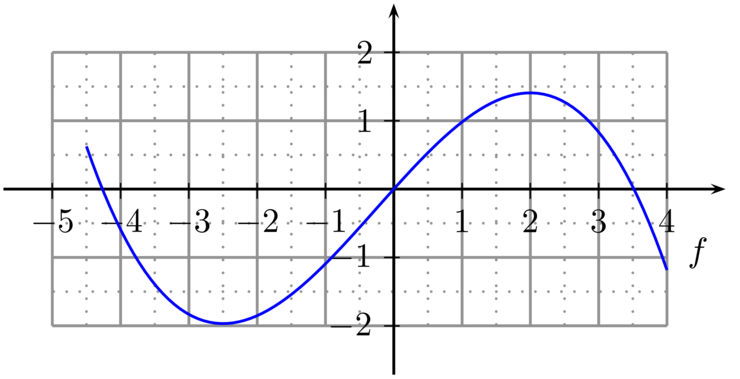
\includegraphics{Picture_FIGLabelFigExVariationRXTkocPICTExVariationRXTkoc-for_eps.pdf}
%The result is on figure \ref{LabelFigExVariationRXTkoc}.
%\newcommand{\CaptionFigExVariationRXTkoc}{<+Type your caption here+>}
\input{Fig_ExVariationRXTkoc.pstricks}

\end{multicols}


\subsection{Définition}

\begin{definition}
      Soit $f$ une fonction définie sur $\defD$ et $I$ un
      intervalle de $\defD$.\\[-2ex]
      \begin{enumerate}
          \item On dit que $f$ est \defe{croissante}{croissante (fonction)} sur $I$
        si et seulement si pour tous réels $a$ et $b$ de $I$, 
        si $a\leq b$ \ alors \ $f(a)\leq f(b)$.
    \item On dit que $f$ est \defe{décroissante}{décroissante (fonction)} sur $I$
        si et seulement si pour tous réels $a$ et $b$ de $I$, 
        si $a\leq b$ \ alors \ $f(a)\geq f(b)$. 
      \end{enumerate}
\end{definition}


\begin{remark}
    Une fonction croissante range les images dans le même ordre que les antécédents. Une fonction décroissante inverse cet ordre. 
\end{remark}


\begin{definition}
    On dit que $f$ est \defe{strictement croissante}{strictement croissante} sur~$I$
  si pour tous réels $a$ et $b$ de $I$ tels que $a<b$, on a $f(a)<f(b)$.

  La fonction \( f\) est \defe{strictement décroissante}{strictement décroissante} sur \( I\) si pour tous réels $a$ et $b$ de $I$ tels que $a<b$, on a $f(a)>f(b)$.
\end{definition}
La différence entre la croissance et la \emph{stricte} croissance est que l'inégalité est stricte.

\begin{definition}
    Soit \( I\) un intervalle de \( \eR\). Nous disons que la fonction \( f\) est \defe{monotone}{monotone} sur $I$ si elle est soit croissante sur $I$, soit décroissante sur $I$.
\end{definition}

\begin{multicols}{2}

    La fonction dessinée ci-contre n'est pas monotone sur l'intervalle \( \mathopen[ -2 , 0 \mathclose]\). Elle est
    \begin{itemize}
        \item 
            monotone décroissante sur \( \mathopen[ -2.5 , -1 \mathclose]\);
        \item
            monotone croissante sur \( \mathopen[ -1 , 1 \mathclose]\);
        \item
            monotone décroissante sur \( \mathopen[ 1 , 1.5 \mathclose]\).
    \end{itemize}

\columnbreak

%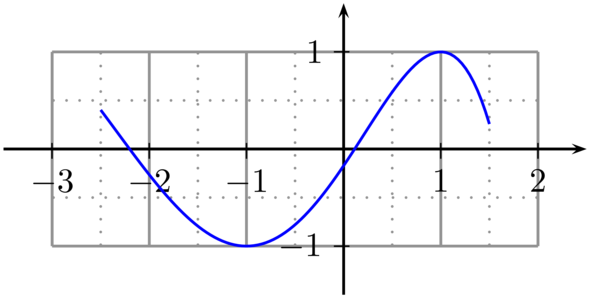
\includegraphics{Picture_FIGLabelFigGrapheVarndvdQMPICTGrapheVarndvdQM-for_eps.pdf}
%The result is on figure \ref{LabelFigGrapheVarndvdQM}.
%\newcommand{\CaptionFigGrapheVarndvdQM}{<+Type your caption here+>}
\input{Fig_GrapheVarndvdQM.pstricks}

\end{multicols}




\begin{definition}
    Soit \( I\) un intervalle. On dit que $f$ est \defe{constante}{constante (fonction)} sur $I$ lorsque pour tous les réels $a$ et $b$ de $I$, on a $f(a)=f(b)$. (Tous les réels de $I$ ont la même image par $f$).
\end{definition}

\begin{multicols}{2}
    Dans ce cas, il existe $k\in\eR$ tel que pour tout $a\in I$, $f(a)=k$. 
    
    La figure ci-contre donne le graphe de la fonction \( f(x)=1.5\) entre \( x=-3\) et \( x=3\).

\columnbreak

%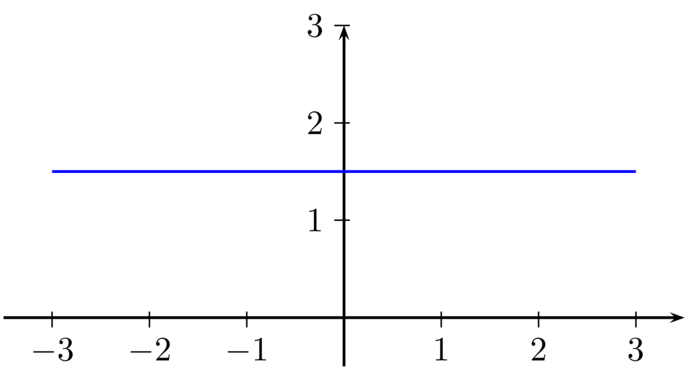
\includegraphics{Picture_FIGLabelFigFoncConstFdDkhWPICTFoncConstFdDkhW-for_eps.pdf}
%The result is on figure \ref{LabelFigFoncConstFdDkhW}.
%\newcommand{\CaptionFigFoncConstFdDkhW}{<+Type your caption here+>}
\input{Fig_FoncConstFdDkhW.pstricks}

\end{multicols}


\subsection{Sens de variation d'une fonction affine}

\begin{Aretenir}
      Soit $f$ la fonction affine $x\mapsto ax+b$.
      \begin{itemize}
      \item Si $a>0$, alors $f$ est croissante sur $\eR$.
      \item Si $a<0$, alors $f$ est décroissante sur $\eR$.
      \item Si $a=0$, alors $f$ est constante sur $\eR$
        (et $f(x)=b$ pour tout $x\in\eR$).
      \end{itemize}
\end{Aretenir}
Nous savons que si \( f(x)=ax+b\), alors \( f\) s'annule en \( x=-\frac{ b }{ a }\). Cela nous sert à écrire un tableau de signe de \( f\).



Les figures \ref{LabelFigFnAffineipcEQfssLabelSubFigFnAffineipcEQf0} et \ref{LabelFigFnAffineipcEQfssLabelSubFigFnAffineipcEQf1} montrent des droites affines. Lorsque \( a>0\), la droite monte; lorsque \( a<0\) elle descend. La pente est d'autant plus forte que \( a\) est grand.
\newcommand{\CaptionFigFnAffineipcEQf}{Deux droites affines.}
\input{Fig_FnAffineipcEQf.pstricks}


\begin{Aretenir}
      Règle du signe de $ax+b$ \\
      
      \begin{tabular}{cc}
        $a<0$ & $a>0$ \\
        & \\
        $\begin{array}{|c|ccccc|}
          \hline
          x & -\infty & & -\dfrac{b}{a} & & +\infty \\[2ex]
          \hline
          ax+b & & + \quad \ & 0 & \quad - & \\[1ex]
          \hline
        \end{array}$
        &
        $\begin{array}{|c|ccccc|}
          \hline
          x & -\infty & & -\dfrac{b}{a} & & +\infty \\[2ex]
          \hline
          ax+b & & - \quad \ & 0 & \quad + & \\[1ex]
          \hline
        \end{array}$ \\
      \end{tabular}  \\[1ex] 
\end{Aretenir}

\subsection{Tableau de variations}


Le \defe{tableau de variation}{tableau de variation} est un tableau contenant
\begin{enumerate}
    \item
        les positions des sommets,
    \item
        les flèches indiquant les endroits où la fonction est croissante ou décroissante.
\end{enumerate}
Un petit exemple valant mieux qu'un long discours\ldots

% à noter le 9 dans l'environnement suivant est le nombre de lignes sur lesquelles la figure s'étale. Je suis obligé de donner à la main parce que le tableau ne compte apparemment que pour une seule ligne. Du coup si je laisse à LaTeX le soin de calculer, les lignes de texte en-dessous de la figure (et en particulier à la page suivante si la figure est en bas de page) sont encore coupées.
\begin{wrapfigure}[9]{r}{6.0cm}     
   \vspace{-1cm}        % à adapter.
   \centering
   \input{Fig_GrapheVarREGMqx.pstricks}
\end{wrapfigure}

    Le tableau de variation de la fonction dessinée ci-contre est :
    \begin{equation*}
    \begin{array}[h]{|c|ccccccc|}
        \hline
        x&-3&&-2&&0&&2\\
        \hline
        &&&2&&&&1\\
        f(x)&&\nearrow&&\searrow&&\nearrow&\\
        &-\frac{ 9 }{2}&&&&-\frac{ 1 }{2}&&\\
        \hline
    \end{array}
    \end{equation*}
    En effet, la fonction \( f\)
    \begin{itemize}
        \item 
            part de \( x=-3\) où \( f(x)=-9/2\);
        \item
            elle monte jusqu'en \( x=-2\) où elle vaut \( f(x)=2\);
        \item
            elle descend jusqu'en \( x=0\) où elle vaut \( -\frac{ 1 }{2}\);
        \item
            elle monte jusqu'en \( x=2\) où elle vaut \( 1\).
    \end{itemize}

Le plus souvent si on donne un dessin, les nombres à placer dans un tableau de variation sont des valeur approchées à la précision du dessin. Donner les réponses en fraction n'est donc pas obligatoire. Par exemple ici au lieu d'écrire \( -9/2\) dans le tableau, il aurait été possible d'écrire \( -4.5\).

\section{Minimum et maximum}

Les notions de minima et maxima parlent, comme l'indiquent leurs noms en français, des points du graphe d'une fonction les plus hauts et les plus bas.

\begin{definition}
      Soit $f$ une fonction définie sur un intervalle $I$.
      \begin{itemize}
          \item On dit que $f$ admet le réel $m$ pour \defe{minimum}{minimum (d'une fonction)} sur $I$ si et seulement si il existe $c\in I$ tel que $f(c)=m$ et pour tout $x\in I$, $f(x)\geq m$. 
    \item On dit que $f$ admet le réel $M$ pour \defe{maximum}{maximum} sur $I$ si et seulement si il existe $d\in I$ tel que $f(d)=M$ et pour tout $x\in I$, $f(x)\leq M$.
      \end{itemize}
\end{definition}

Sur la figure \ref{LabelFigMinMaxKNRdOd}, nous avons indiqué le minimum et le maximum de la fonction dessinée.
\newcommand{\CaptionFigMinMaxKNRdOd}{Minimum et maximum d'une fonction.}
\input{Fig_MinMaxKNRdOd.pstricks}


%+++++++++++++++++++++++++++++++++++++++++++++++++++++++++++++++++++++++++++++++++++++++++++++++++++++++++++++++++++++++++++ 
\section{Exercices : généralités sur les fonctions}
%+++++++++++++++++++++++++++++++++++++++++++++++++++++++++++++++++++++++++++++++++++++++++++++++++++++++++++++++++++++++++++

%---------------------------------------------------------------------------------------------------------------------------
\subsection{Image, antécédent}
%---------------------------------------------------------------------------------------------------------------------------

\Exo{Seconde-0042}
\Exo{Seconde-0048}
\Exo{Seconde-0054}
\Exo{Seconde-0051}
\Exo{Seconde-0050}

%---------------------------------------------------------------------------------------------------------------------------
\subsection{Exemples de fonctions}
%---------------------------------------------------------------------------------------------------------------------------

\Exo{Seconde-0058}
\Exo{Seconde-0057}
\Exo{Seconde-0063}
\Exo{Seconde-0061}
\Exo{Seconde-0067}
\Exo{smath-0295}

%---------------------------------------------------------------------------------------------------------------------------
\subsection{Représentation graphique}
%---------------------------------------------------------------------------------------------------------------------------

\Exo{Seconde-0043}
\Exo{Seconde-0059}
\Exo{Seconde-0047}
\Exo{Seconde-0060}
\Exo{Seconde-0049}

\Exo{smath-0127}
\Exo{smath-0439}

%---------------------------------------------------------------------------------------------------------------------------
\subsection{Travail sur les graphiques}
%---------------------------------------------------------------------------------------------------------------------------

\Exo{Seconde-0069}
\Exo{Seconde-0070}
\Exo{Seconde-0071}

% TODO : ce serait pas mal de mettre une question pleine de texte ici.

\Exo{smath-0015}
\Exo{Seconde-0072}
\Exo{smath-0209}
\Exo{smath-0298}

%---------------------------------------------------------------------------------------------------------------------------
\subsection{Problèmes et résolution d'équation}
%---------------------------------------------------------------------------------------------------------------------------


\Exo{smath-0210}
\Exo{smath-0001}
\Exo{smath-0004}
\Exo{smath-0005}
\Exo{smath-0006}
\Exo{Seconde-0046}

\Exo{smath-0186}    % Cet exercice est le même que le smath-0111, mais vu différemment.
\Exo{smath-0078}
\Exo{smath-0013}
\Exo{Seconde-0068}
\Exo{Seconde-0064}
\Exo{Seconde-0044}
\Exo{Seconde-0066}
\Exo{Seconde-0075}
\Exo{Seconde-0076}

%---------------------------------------------------------------------------------------------------------------------------
\subsection{Plus avancés}
%---------------------------------------------------------------------------------------------------------------------------

\Exo{Premiere-0018}
